\section{Summary of results and price-performance}\label{resultsSummary}

In this section we summarize the results obtained using the different configurations presented previously. We discuss the total execution times and monetary costs. Additionally, we introduce an adapted version of the TPC-DS metric to facilitate performance comparisons, which enables us to derive price-performance criteria. Finally, we estimate the cost effects of opting for spot EC2 instances instead of on-demand instances.

\subsection{Total execution times}\label{resultsSummaryTotalExecutionTimes}

Figure \ref{fig:resultsSummaryTotalTimes} presents the total time required for executing the TPC-DS Benchmark at the 1 TB scale factor for the different configurations that we have covered. The total times are composed from the Data Loading Test, the Power Test, and the Throughput Test times. By far the largest component is the Throughput Test in all cases.

\begin{figure}
   \begin{center}
   \scalebox{0.75}{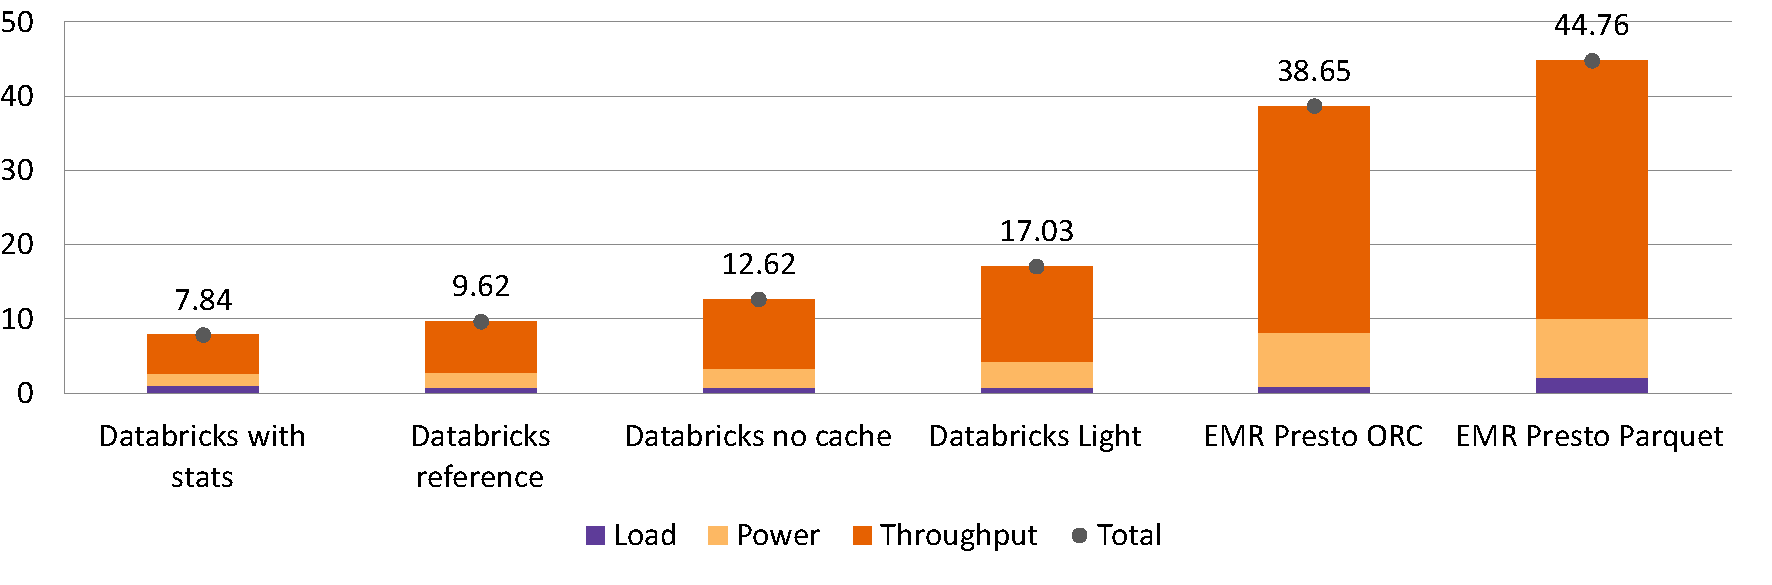
\includegraphics[width=7.0in]{imgs/resultsSummary/TotalTimes.pdf}}
   \end{center}
   \caption{TPC-DS Benchmark total execution time for various configurations.}
   \label{fig:resultsSummaryTotalTimes}
\end{figure}

The lowest total time is achieved with Databricks using the cost-based optimizer with table and column statistics. It represents an almost 5 times faster alternative than the most efficient configuration for EMR Presto. In the case of Databricks Data Engineering without the cost-based optimizer, our reference configuration, the advantage drops to about 4 times faster, still very significant. Notably, Databricks Light and EMR Presto using the ORC format show very similar performance.

\subsection{Total costs}\label{resultsSummaryTotalCost}

Regarding the monetary costs incurred to obtain the total execution times listed above, we present them in Figure \ref{fig:resultsSummaryTotalCosts}.

\begin{figure}
   \begin{center}
   \scalebox{0.75}{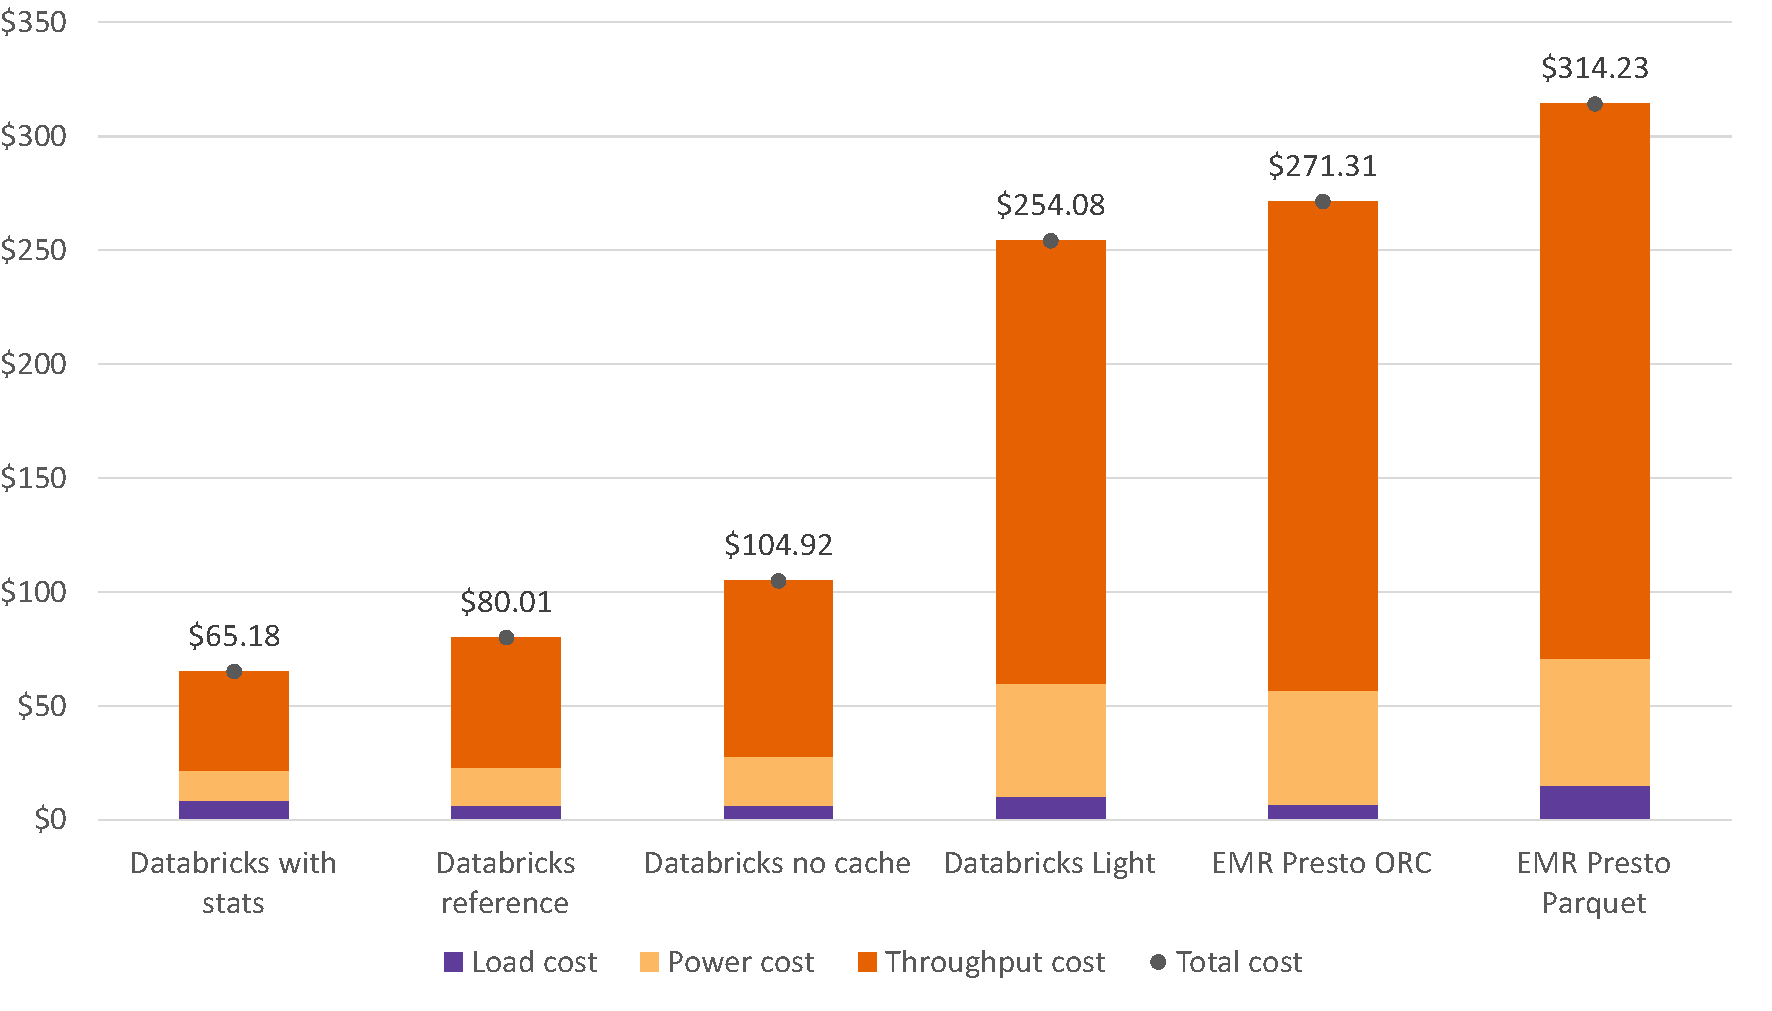
\includegraphics[width=7.0in]{imgs/resultsSummary/TotalCosts.pdf}}
   \end{center}
   \caption{TPC-DS Benchmark total execution time for various configurations.}
   \label{fig:resultsSummaryTotalCosts}
\end{figure}

Again, we obtain the lowest cost with Databricks with table and column statistics, which is over 4 times cheaper than EMR Presto using ORC. When comparing the reference Databricks configuration with EMR Presto using ORC, it is about 3.4 times cheaper. In turn, Databricks Light is not only slightly faster than EMR Presto ORC, but also cheaper.

Disabling the io cache for Databricks increases the cost significantly, therefore it is a feature that provides real benefits. Nevertheless, additional experiments would be required to determine whether if using lower cost EC2 instances not optimized for io, and potentially inviable for the io cache, could yield a lower cost. For example, the memory optimized r5.2xlarge instances offer the same 8 cores with 3 additional GB of memory, but no NVMe SSD at a cost of \$0.504. Assuming the total time obtained with these instances would be the same as with the cache disabled, the total cost would be \$91.29, still greater than the \$80.01 cost with Databricks Data Engineering with cache enabled, our reference configuration.

The prices shown above employ on-demand EC2 instances. Amazon Web Services offers an alternative pricing model for EC2 instances called spot instances. These represent spare computing capacity that AWS makes available at heavily discounted prices, but whose availability can vary greatly during the year and across the various regions. Furthermore, such changes in availability can trigger spot instance interruptions, which the application should be prepared to handle.

We next estimate the costs of employing spot instances instead of on-demand instances. We base our calculations on the Spot Instance Advisor\footnote{https://aws.amazon.com/ec2/spot/instance-advisor/}, which estimates savings based on data covering the last 30 days. For the i3.2xlarge instances that we use for both our Databricks and EMR Presto deployments, running in the US West (Oregon) region, the savings are reported to be 70\% and the frequency of interruption less than 5\%. This results in the costs we show in Figure \ref{fig:resultsSummaryTotalCostsWithDiscount}.

\begin{figure}
   \begin{center}
   \scalebox{0.75}{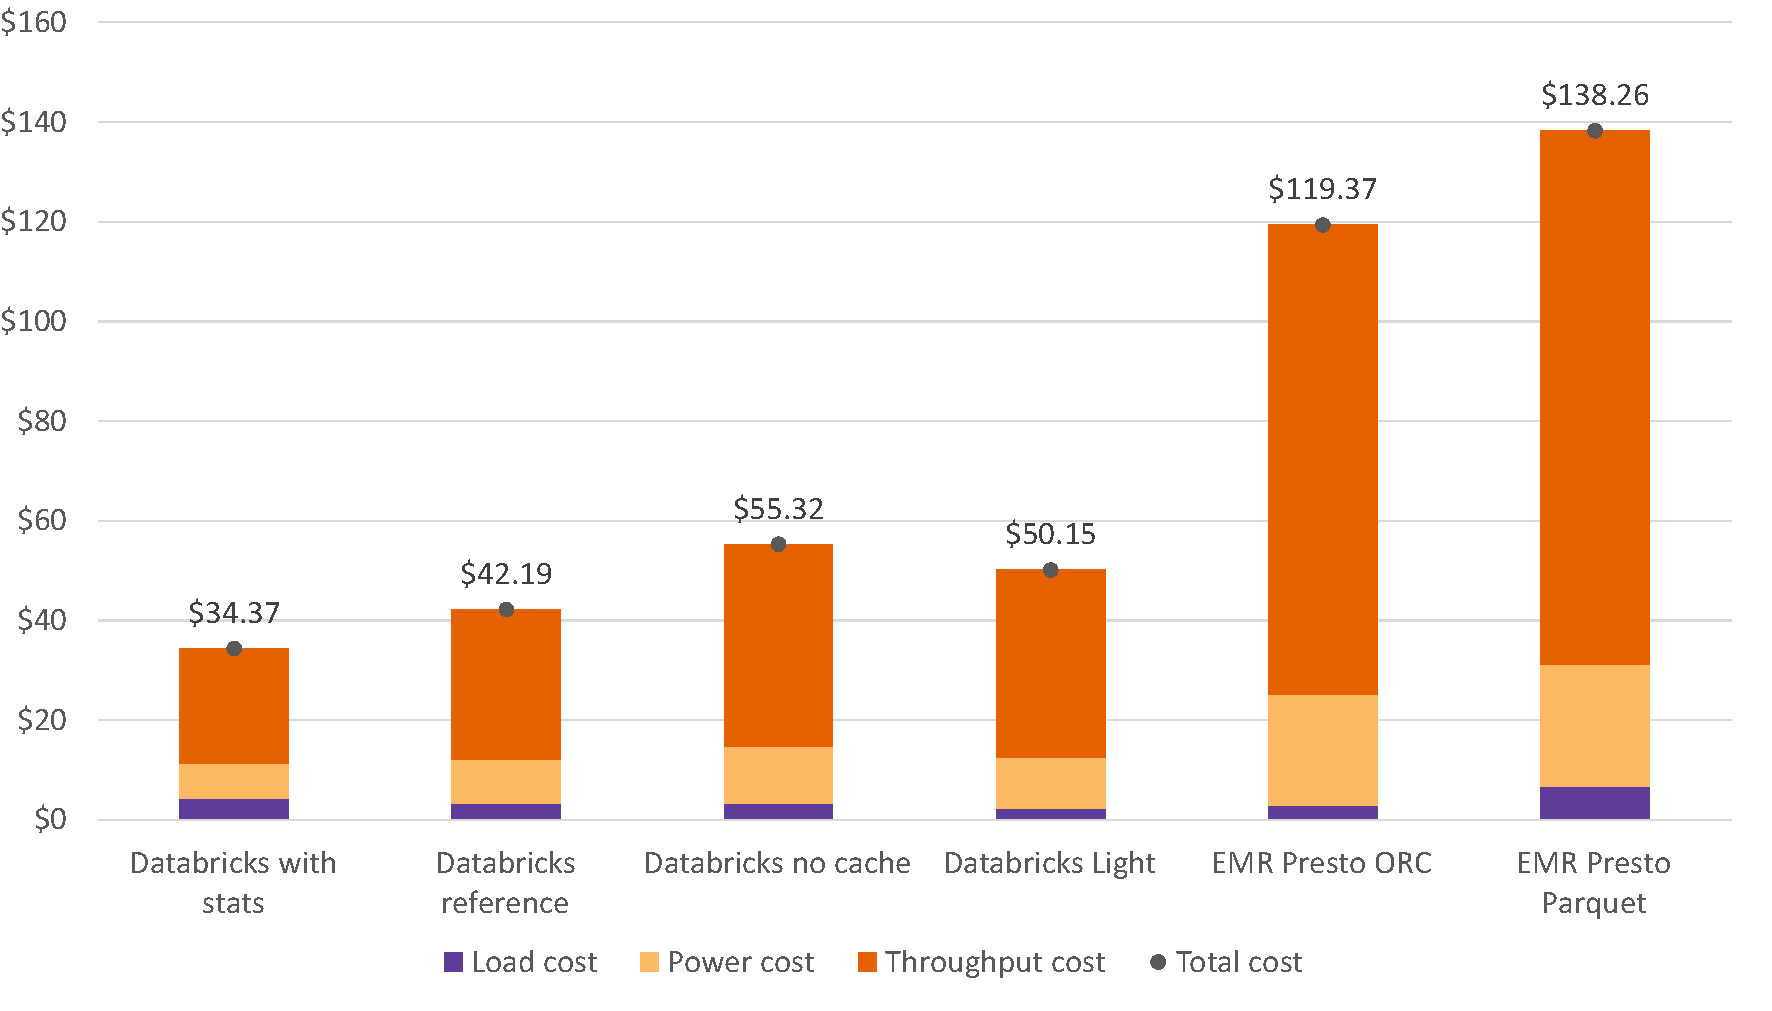
\includegraphics[width=7.0in]{imgs/resultsSummary/TotalCostsWithDiscount.pdf}}
   \end{center}
   \caption{Estimated TPC-DS Benchmark total cost for various configurations using spot EC2 instances.}
   \label{fig:resultsSummaryTotalCostsWithDiscount}
\end{figure}

The costs are reduced by more or less about half. Since the Databricks Data Engineering software costs now dominate the node cost per hour, the Databricks reference costs compared to the EMR Presto ORC costs now are about 2.8 times cheaper instead of 3.4 times cheaper, still a difference of great magnitude.

\subsection{TPC-DS performance metric}\label{resultsSummaryPerformanceMetric}
